\documentclass{article}
\usepackage{graphicx}
\usepackage[spanish]{babel}
\usepackage[utf8]{inputenc} % Ensures proper handling of special characters
\usepackage{amsthm}
\usepackage{amsmath}
\usepackage{amsfonts}
\usepackage[font=footnotesize,labelfont=bf,labelsep=colon]{caption} % Personalización de captions
\DeclareMathOperator*{\argmin}{arg\,min}
% Define the unnumbered theorem
\newtheorem{thm}{Teorema}[section]
\newtheorem{dfn}{Definición}[section]
%\newtheorem*{def}{Definicion}

\begin{document}


\title{Teoría del Aprendizaje Estadístico}
\author{Nicolas Silva Nash \\ Departamento de Matemática \\ Universidad Nacional del Comahue}
%\date{\today}
\maketitle

\section{Introducción}
La Teoría del Aprendizaje Estadístico proporciona la base teórica para muchos de los algoritmos de aprendizaje automático actuales y,
sin lugar a dudas, es una de las ramas más bellamente desarrolladas de la inteligencia artificial en general. Nació con el perceptrón de Rossenblat
y la escuela matemática de la Unión Soviética en la década de 1960, y ganó amplia popularidad en la década de 1990 tras el desarrollo de las llamadas 
Máquinas de Vectores de Soporte (\textit{SVM}, por sus siglas en inglés), que se han convertido en una herramienta estándar para el reconocimiento de 
patrones en muchas disciplinas, que van desde la visión por computadora hasta la biología computacional.\\

Proporcionar la base para nuevos algoritmos de aprendizaje no ha sido la única motivación para desarrollar la Teoría del Aprendizaje 
Estadístico. También ha sido una gesta de caracter filosófico, en el intento de responder a la pregunta de qué nos permite extraer conclusiones válidas 
a partir de datos empíricos.  

\section{El aprendizaje}

En este contexto, el \textit{aprendizaje} es el proceso a través del cual pueden inferirse reglas generales a partir de ejemplos. Nos interesa 
entender como una máquina -una computadora- puede resolver ciertos problemas sin conocer las reglas de antemano, solo a partir de ejemplos y a través
de un \textit{algoritmo de aprendizaje}. El objetivo es que la máquina pueda no solo aprender a reconocer las reglas que rigen a los ejemplos dados,
si no que también pueden generalizar dichas reglas para ejemplos que le serán presentados con posterioridad.\\

Llamamos a esta disciplina \textit{aprendizaje automático} (en inglés, \textit{Machine Learning}, literalmente ``aprendizaje de máquinas") y reconocemos
sus raíces en otras disciplinas: Estadística Matemática, Ciencias de la Computación e Inteligencia Artificial. Si bien el aprendizaje suele ser una
parte fundamental de la mayoría de los esfuerzos en materia de Inteligencia Artificial, el objetivo del Machine Learning es más acotado que el de su 
rama madre: En vez de intentar definir, explicar o generar comportamiento inteligente o \textit{inteligencia}, aquí nos interesa solamente descubrir los mecanismos
a través de los cuales las computadoras pueden resolver algunas tareas acotadas y bien definidas, y que en general escapan a soluciones que pueden
ser especificadas con una cantidad finita de código de programación (reglas determinísticas). \\

Con fines ilustrativos, nos centraremos primero en el más conocido de los problemas del Machine Learning, el de clasificación. Consideremos dos espacios
de variables: \(X\), llamado \textit{espacio de entrada}, e \(Y\), el  \textit{espacio de etiquetas}. En un problema de clasificación, deseamos poder etiquetar
correctamente elementos de \(X\) con los valores de \(Y\). Por ejemplo, podríamos querer clasificar un conjunto de datos, en alguna representación fija, de distintos 
objetos en una cantidad de etiquetas como: silla, cama, microondas, perro, gato. Si esta representación es en imágenes de \(N\times M\) pixeles en blanco y negro (realmente, 
matrices de orden \(N\times M\) con coeficientes reales en el interavalo \([0,1]\) que representan la intensidad de cada pixel, del negro al blanco), el espacio \(X\) es 
el conjunto de dichas matrices y el espacio \(Y\) las categorías distintas que corresponden a lo que las imágenes muestran. Con el fin de aprender, a un algoritmo se le 
muestran ejemplos de imágenes y sus respectivas etiquetas \((X_1,Y_1)\), \((X_2,Y_2)\), ..., \((X_n,Y_n)\), a partir de los cuales este debe encontrar una función
\(f: X\rightarrow Y\), que comete la menor cantidad de errores posibles. A esta función \(f\) la llamamos \textit{clasificador}.

\section{La historia del aprendizaje automático}

El primer modelo de aprendizaje automático, según Vapnik en [2], fue sugerido por F. Rosenblatt, un psicólogo estadounidense, al que llamó \textit{perceptrón}, y su introducción
constituye el comienzo del análisis matemático del aprendizaje. Conceptualmente, la idea del perceptrón no era nueva, estando presente en la litetura de Neurofisiología durante
varios años. Rosenblatt, sin embargo, se aventuró en describir el modelo como un programa para computadoras y demostró con simples experimentos que dicho modelo era generalizable.
El perceptrón fue construído como una solución a un problema particular dentro del aprendizaje automático, el reconocimiento de patrones. En el caso más sencillo, este problema
consiste en hallar una regla para separar datos en dos categorías distintas a partir de ejemplos.\\

Para construir la regla de separación, el perceptrón sigue el modelo más sencillo de neurona, propuesto previamente por McCulloch y Pitts, de acuerdo al cual una neurona recibe
\(n\) valores (o \textit{inputs}) en la forma de un vector \(x = (x^1,\dots, x^n) \in X \subset \mathbb{R}^n \) y genera una etiqueta (\textit{output}) 
\(y\in\{-1,+1\}\) a través de una dependecia funcional dada por
\[
y = sgn\{(w\cdot x)-b\}
\]

con \(\cdot\) el producto interno de vectores en \(\mathbb{R}^n\), \(b\) un valor de límite y un vector \(w\) que se genera en el proceso de aprendizaje. Geométricamente, una 
neurona divide el espacio \(X\) en dos regiones: en una la etiqueta \(y\) vale \(+1\) y en la otra \(-1\). Las dos regiones son separadas por el hiperplano:
\[
(w\cdot x) - b = 0
\]


El vector \(w\) y el escalar \(b\) determinan la posición del hiperplano y sus valores son aprendidos por el perceptrón. Cuando combinamos varias neuronas, el perceptrón
separa el espacio de entrada en en dos regiones lineales a trozos y no necesariamente conexas. En 1960 no era claro como elegir todos los parametros \((w_1,\dots,w_k)\) y
\((b_1,\cdots, b_k)\) de todas las neuronas, por lo que se fijaban los valores de las primeras \(k-1\) y se intentaba encontrar los valores deseables para la última
de ellas. Geométricamente, se transformaba el espacio de entrada $X$ en un nuevo espacio $Z$ (eligiendo coeficientes apropiados para las primeras $k-1$ neuronas) y luego
se utilizaban los datos de entrenamiento para construir un hiperplano que separe el plano $Z$.
Tomando prestados de la fisiología los conceptos de aprendizaje con estímulos de premios y castigos, Rosenblat propuso un simple algoritmo para hallar estos 
coeficientes de manera iterativa, el cual describiremos a continuación.

DESCRIBIR perceptrón.\\

En 1962 Novikoff demostró el primer teorema relacionado al perceptrón. Podemos decir que este teorema inció propiamente la teoría del aprendizaje.

\begin{thm}
Dado un conjunto de datos de entrenamiento como el descrito previamente, de manera que\\
1) La norma de los vectores de entrenamiento $z_i$ está acotada por una constante $R$:
$$
|z_i| \leq R, \qquad \forall i=1,2,\dots,k
$$
2) Los datos de entrenamiento pueden separados con un margen $\rho$:
$$
\sup_{w} \min_{i} y_i(z_i\cdot w) > \rho
$$
3) Los datos son alimentandos al perceptrón una cantidad \textit{suficiente} de veces.\\

Entonces el algoritmo encuentra el hiperplano que separa los datos de entrenamiento, luego de a lo
sumo $N$ correcciones, con $N$ verificando:
$$
N \leq \left [ \frac{R^2}{\rho^2}\right ]
$$

\end{thm}

Resaltamos este teorema porque jugó un papel fundamental en la creación de la teoría del aprendizaje, conectando el
principio de minimización de errores en el conjunto de datos de entrenamiento con la capacidad de generalización
de los algoritmos de clasificación y su causa.

\section{Hacia la formalización}

Volviendo al caso de clasificación binaria en aprendizaje supervisado, partimos de ejemplos (datos de entrenamiento) 
en un espacio de entrada $X$ con alguna de las dos posibles etiquetas del espacio $Y=\{-1,+1\}$. Aquí, \textit{aprender}
se reduce a estimar una relación funcional $f:X\rightarrow Y$, el clasificador. Un algoritmo de aprendizaje es aquel
que a partir de los datos de entrenamiento construye una función $f$. Nos interesa construir una teoría que no asuma
de manera estricta nada acerca de $X$ e $Y$, pero nos permitimos asumir ciertas cosas del mecanismo que genera los
datos de entrenamiento. En particular, asumiremos que existe una \textit{distribución de probabilidad conjunta} $P=P(X,Y)$
sobre $X\times Y$ y que las muestras son tomadas de forma independiente de esta distribución de forma \textit{iid} -independiente
e idénticamente distribuída-. Notemos lo siguiente:
\begin{enumerate}
    \item \textit{No imponemos condiciones a la distribución de probabilidad $P$}. La gran diferencia que encontramos entre la Estadística
    tradicional y la teoría del aprendizaje estadístico es que en esta última trabajamos de manera agnóstica a la distribución
    que genera las muestras y deseamos llegar a conclusiones generales.
    \item \textit{Consideramos a las etiquetas de manera no determinística.} Consideramos a $P$ como una distribución de probabilidad
    no solo sobre las instancias de $X$, si no también sobre las propias etiquetas de $Y$. Por lo tanto, estas últimas no son solo 
    funciones tradicionales de los datos en $X$, si no que ellas mismas pueden ser aleatorias. Tenemos al menos dos buenas razones
    para tomar esta consideración: por un lado, el proceso de generación de datos puede tener ruido al asignar etiquetas (por ejemplo
    tomemos el caso de un detector de spam basado en la opinión de etiquetadores humanos que clasifican emails con un porcentaje de error; incluso
    los humanos pueden clasificar incorrectament algunos de esos emails), y por otro, ciertos problemas se prestan a que existan
    clases que se solapan (pensemos en la dificultad en diferenciar a un perro de un gato en una fotografías que los captura desde
    una gran distancia o con baja resolución).\\
    En la práctica, en vez de asignar etiquetas a los elementos en $X$ de manera determinística, daremos la probabilidad condicional
    de la etiqueta $y$ dado el valor $x$. En el caso de clasificación binaria, basta solo dar la probabilidad $P(Y=1|X=x)$ de que la etiqueta
    tenga valor $Y=1$, dado que la restante es complementaria:
    $$
    P(Y=-1|X=x) \quad = \quad 1 - P(Y=1|X=x)
    $$
    Ciertos problemas que hagan uso de datos con etiquetas con poco ruido nos llevaran naturalmente a probabilidades condicionales cercanas
    a $0$ y $1$, dejando un margen de error pequeño, pero cuando tratemos con solapamiento de clases, las probabilidades condicionales
    pueden acercarse a $\frac{1}{2}$ para cada etiqueta. Independientemente de la causa, que las probabilidades condicionales sobre
    las etiquetas se acerquen a $\frac{1}{2}$ vuelve más dificil el aprendizaje, dado que crece el número de errores del clasificador.
    \item \textit{Muestro independiente}. Una de las condiciones más fuertes que imponemos en la teoría del aprendizaje estadístico es
    que asumimos que las muestras son tomadas de forma independiente. En muchas aplicaciones, esta suposición está justificada, pero
    hay ramas muy importantes de la disciplina en donde esto no se cumple, por ejemplo en el análisis de series de tiempo, en donde
    la secuencialidad de los datos viola la condición de iid (cada valor depende en alguna medida de los anteriores). Esto es también 
    cierto para las aplicaciones a lenguaje natural, y constituye una de las razones principales por las cuales esta rama más moderna 
    del aprendizaje tiene bases teóricas menos fuertes que el aprendizaje automático tradicional.
    \item \textit{La distribución P es fija}. Al no considerar al tiempo como un parámetro, ni existir un orden en las muestras, asumimos
    que la distribución que las origina es siempre la misma. Esto, como en el punto anterior, no se cumple en las series de tiempo. Otro
    caso donde se viola esta suposición es en aquellos problemas en donde la distribución de probabilidad de los datos de entrenamiento no
    coincide con el de los datos posteriores, llamado \textit{covariate shift}, por ejemplo en un sistema de \textit{scoring} de usuarios
    de una empresa que crece súbitamente y que suma a personas que no se corresponden a los perfiles que existían originalmente en su base
    de datos (e.g. se admite que inmigrantes no bancarizados y sobre los que no hay datos previos accedan a préstamos).
    \item \textit{La distribución P es desconocida al momento de aprender}. Si conociéramos de antemano la probabilidad condicional $P$,
    el problema del aprendizaje sería trivial pues podríamos siempre determinar el mejor clasificador posible (aunque no sea perfecto,
    dada la naturaleza aleatoria de las etiquetas). Solo tenemos acceso a $P$ de manera indirecta, a través de las muestras. Intuitivamente,
    esto nos hace pensar que, consiguiendo un número lo suficientemente grande de muestras, podemos aproximar las propiedades de la distribución
    $P$, pero con errores. Uno de los principales logros de la teoría del aprendizaje estadístico es brindarnos un marco teórico para
    acotar este error.
\end{enumerate}

\subsection{Pérdida y Riesgo}

Para saber qué tan bien se comporta un clasificador $f$, necesitamos medir sus equivocaciones. Para esto, definiremos una \textit{función de pérdida},
$\ell$, que le asigne un valor al hecho de que $f$ clasifique a cierto $x\in X$ con la etiqueta $y\in Y$. Llamermos \textit{costo} a dicho valor, 
dado que más adelante penalizaremos al clasificador en base a los errores que cometa a través del alogritmo de aprendizaje.\\
El ejemplo más sencillo de función de pérdida es la ``pérdida-0-1'', que le asigna un costo de $0$ a una instancia de clasificación correcta y un costo
$1$ a una incorrecta, es decir:
$$
\ell(X,Y,f(X)):= \begin{cases}
    1 \qquad \text{si } f(X) \neq Y \\
    0 \qquad \text{si } f(X) = Y
\end{cases}
$$
En problemas de regresión, la función de pérdida más conocida es el \textit{error cuadrático}, dado por
$$
\ell(X,Y,f(X)):= (Y-f(X))^2
$$
Por convención, una pérdida igual a $0$ implica una clasificación perfecta y valores mayores implican peor clasificación. Es decir,
el aprendizaje suele implicar un desafío de optimización en dónde deseamos hallar el mínimo de la función de perdida.

Mientras que la función de pérdida mide el error del clasificador en un punto individual $x\in X$, llamamos \textit{riesgo}, $\mathcal{R}$, 
del clasificador a la pérdida esperada sobre todos los datos generados por la distribución de probabilidad $P$. Es decir
$$
\mathcal{R}(f) := E\left( \ell(X,Y,f(X)) \right)
$$
Desde luego que otra función $g$ es un mejor clasificador que $f$ para un problema dado si su riesgo es más bajo, es decir si $\mathcal{R}(g)
< \mathcal{R}(f)$, por lo que el mejor clasificador de todos es aquel con el riesgo más bajo.\\

Algo que no hemos considerado aún es si los clasificadores $f$ tienen alguna característica especial. Para formalizarlo, tomaremos funciones de un
espacio de funciones $\mathcal{F}$ que aplican $X$ en $Y$. En un principio, parecería aceptable tomar el espacio de todas las funciones posibles, o 
más precisamente, el conjunto de todas las funciones \textit{medibles} que aplican $X$ en $Y$, $\mathcal{F}_{all} = \{f \text{ medibles  } | 
\; f: X \rightarrow Y \}$. En este caso, podemos señalar cuál es el clasificador ideal, dada la distribución $P$, al que llamamos
\textit{clasificador Bayesiano}, $f_{\text{Bayes}}$, y al que definimos como:
$$
f_{\text{Bayes}} := \begin{cases}
1 \qquad \; \; \text{  si } P(Y=1 | X=x) \geq \frac{1}{2}\\
-1 \qquad \text{en otro caso }
\end{cases}
$$

Observermos que, en caso de que las etiquetas fueran determinísticas, es decir donde $P(Y=y|X=x)=1$ para cada $x\in X$ con su
respectiva etiqueta $y$, $f_{\text{Bayes}}$ eligiría correctamente en todos los casos. De existir un ligero solapamiento de clases 
de tal manera que para un cierto $x$ tengamos $P(Y=1|X=x) = 0.9$, entonces tendríamos
que en la mayoría de los casos la etiqueta de $x$ es $+1$ y, siendo este el valor elegido por $f_{\text{Bayes}}$, el clasificador
Bayesiano estaría en lo correcto.\\

En la práctica no es posible computar directamente el clasificador Bayesiano dado que, como dijimos, la distribución de probabilidad
conjunta $P$ es desconocida. Sin embargo, este clasificador es una herramienta teórica que nos permite formular el problema
estandar de la clasificación binaria, el cual es:\\

\textit{Dado un conjunto de datos de entrenamiento $ \{ (X_1,Y_1),\dots,(X_n, Y_m)\}$ obtenidos iid de una distribución $P$, y dada una
función de pérdida $\ell$, deseamos construir una funión clasificadora $f:X\rightarrow Y$ cuyo riesgo $\mathcal{R}(f)$ sea lo
más cercano posible al riesgo de $f_{\text{Bayes}}$.}\\

Notemos que no solo es imposible computar el error del clasificador Bayesiano, sino también el propio riesgo de cualquier clasificador
$f$. Es decir, dado un problema definido (minimizar el riesgo del clasificador), con una solución ideal que podemos escribir (el propio
clasificador Bayesiano), no tenemos manera de computar ninguna cosa de utilidad. Aquí es donde la teoría de aprendizaje estadístico
nos permite llegar a resultados y obtener garantías de la utilidad de esas soluciones.

\subsection{Generalización}

Dado que no conocemos la distribución de probabilidad $P(X,Y)$, no podemos calcular la esperanza de la pérdida de un clasificador cualquiera
$f$, es decir su riesgo. Lo que si podemos hacer, dado un conjunto de entrenamiento, es ''contar" (o medir, en general, para problemas
que no son de clasificación binaria) el número de errores del clasificador sobre los datos de entrenamiento. A esta cantidad le daremos
el nombre de \textit{riesgo empírico} y lo veremos presente en la literatura también como \textit{error de entrenamiento}. Lo definimos
como
$$
R_{emp}(f) := \frac{1}{n} \sum_{i=1}^n \ell(X_i,Y_i,f(X_i))
$$

Por ejemplo, de la función de pérdida llamada error cuadrático se deriva el riesgo empírico \textit{error cuadrático medio}, que es ampliamente
utilizado en la práctica.

Usualmente, un algoritmo de aprendizaje aceptable es capaz de producir un clasificador $f$ que performa aceptablemente bien en un conjunto de datos
conocido, es decir tal que el riesgo empírico del clasificador es bajo. Nos interesa que un clasificador $f$ tenga riesgo bajo en todo el espacio
de entrada $X$, no solo en los datos de entrenamiento. Decimos que un clasificador \textit{generaliza} bien si la diferencia entre su riesgo
y su riesgo empírico es baja.\\

DEFINICIÓN Generalización\\

Por supuesto que una buena generalización no asegura que el riesgo, ni el riesgo empírico, sean bajos, si no que dichas cantidades son cercanas.
Pero lo que nos interesa es que el riesgo empírico sea un buen estimativo del riesgo del clasificador, y esto es lo que nos permitirá
hacer afirmaciones acerca del error del clasificador en la práctica.

\subsection{Consistencia}
Intuitivamente, parece razonable pedirle a un algoritmo de aprendizaje que, al ser presentado con más y más ejemplos, converja a una
solución óptima. En Estadística, la noción de \textit{consistencia} se relaciona con la capacidad de hacer afirmaciones con respecto a lo que
sucede en el límite de una cantidad infinita de muestras y, a diferencia de la generalización, que es acerca de una función en particular,
es una propiedad de un conjunto de funciones. Para ilustrar este concepto, denotemos como $f_n$ al clasificador construido por un algoritmo
de aprendizaje luego de ser presentado con $n$ puntos de entrenamiento. Por el momento no repararemos en cómo el algoritmo construye esta
función, pero podemos estar seguro que la elige de un cierto espacio funcional $\mathcal{F}$. Más adelante veremos que dicho espacio puede
estar explícitamente dado, como en el caso de la regresión lineal, o no, y existir implícitamente en el mecanismo del propio algoritmo,
como es el caso de las redes neuronales. Más allá de si $\mathcal{F}$ es explícito o no, el algoritmo debe elegir a la mejor función
en dicho espacio basándose en los puntos de entrenamiento. Por otro lado, sabemos precisamente cuál es en teoría el mejor clasificador 
en $\mathcal{F}$: el que tiene el menor riesgo. Por simplicidad, supongamos que este es único (no tiene por qué serlo, puede no haber
un solo mínimo global para la función de riesgo). Definimos a este clasificador óptimo como:
$$
f_{\mathcal{F}} = \argmin _{f\in{\mathcal{F}}} \mathcal{R}(f)
$$
Considerando que el clasificador bayesiano introducido en la sección anterior es el mejor clasificador posible, podríamos denotarlo,
siguiendo la misma convención, como $f_{\mathcal{F}_{all}}$. Desde luego que el espacio $\mathcal{F}$ que elegimos 
puede no contenerlo, por lo que $\mathcal{R}(f_{\text{Bayes}}) < \mathcal{R}(f_{\mathcal{F}})$. Con estas ideas, podemos definir
los distintos de convergencia que trataremos al considerar el concepto de consistencia.

\begin{dfn}
    Sea $(X_i,Y_i)_{i\in\mathbb{N}}$ una sucesión infinita de puntos de entrenamiento que han sido tomados iid de una distribución $P$.
    Sea $\ell$ una función de pérdida. Por cada $n\in \mathbb{N}$, sea $f_n$ un clasificador construído por algún algoritmo de aprendizaje
    usando los primeros $n$ puntos de entrenamiento. Sea $\mathcal{F}$ el espacio funcional de todos los posibles clasificadores según
    el mecanismo de construcción del algoritmo. Entonces
    \begin{enumerate}
    \item  El algoritmo de aprendizaje se dice \textnormal{consistente con respecto a $\mathcal{F}$ y a $P$} si el riesgo $\mathcal{R}(f_n)$
     converge en probabilidad al riesgo  $\mathcal{R}(f_{\mathcal{F}})$ del mejor clasificador en $\mathcal{F}$. Esto es,
     que para todo $\epsilon>0$:
     $$
     P\left(\mathcal{R}(f_n)-\mathcal{R}(f_{\mathcal{F}})>\epsilon\right) \rightarrow 0 \qquad \text{ cuando } \qquad n\rightarrow \infty
     $$ 
     \item  El algoritmo de aprendizaje se dice \textnormal{Bayes-consistente con respecto a $P$} si el riesgo $\mathcal(R)(f_n)$
     converge en probabilidad al riesgo  $\mathcal(R)(f_{\text{Bayes}})$ del clasificador bayesiano. Esto es, para todo $\epsilon>0$
     $$
     P\left(\mathcal{R}(f_n)-\mathcal{R}(f_{\text{Bayes}})>\epsilon\right) \rightarrow 0 \qquad \text{ cuando } \qquad n\rightarrow \infty
     $$ 
    \item  El algoritmo de aprendizaje se dice \textnormal{universalmente consistente con respecto a $\mathcal{F}$} si 
    es consistente con respecto a $\mathcal{F}$ para toda distribución de probabilidad $P$.
    \item  El algoritmo de aprendizaje se dice \textnormal{universalmente Bayes-consistente } si 
    es Bayes-consistente para toda distribución de probabilidad $P$.
    \end{enumerate}
\end{dfn}

Incurrimos en un abuso del lenguaje al decir que "el clasificador $f_n$ es consistente" para referirnos más precisamente a que
"el alogritmo de aprendizaje que produce a $f_n$ en base a las primeras $n$ muestras es consistente". Analicemos un poco más el
significado de las definiciones anteriores. La primer definición nos habla del caso donde, a medida que $n$ crece, el riesgo
del clasificador $f_n$ converge al riesgo del mejor clasificador $f_{\mathcal{F}}$ en el espacio funcional $\mathcal{F}$, con alta probabilidad.
En la práctica, esto significa que alguna instancia de $f_n$ puede no tener un riesgo cercano al riesgo de $f_{\mathcal{F}}$, pero que esto es poco
probable, es decir que de repetir muchas veces el experimento, la mayoría de las veces el riesgo de $f_n$ será cercano al riesgo de $f_{\mathcal{F}}$
a medida que $n$ crece. 

La segunda definición es similar, pero en vez de comparar el riesgo de $f_n$ con el riesgo del mejor clasificador en $\mathcal{F}$,
lo hace con el riesgo del clasificador bayesiano $f_{\text{Bayes}}$. La diferencia es clara, la primera definción se encarga de 
comparar el riesgo de $f_n$ con el mejor clasificador posible dadas las condiciones del aprendizaje, que son las que definen al espacio funcional 
$\mathcal{F}$ (por ejemplo, el mejor clasificador lineal si estamos hablando de regresión lineal), mientras que la segunda lo hace con el
mejor clasificador posible, independientemente de las condiciones del aprendizaje (la función clasificadora ideal podría no ser lineal
para un problema dado).\\

La tercera y cuarta definición son más fuertes, pues piden que el algoritmo sea consistente para cualquier distribución de probabilidad $P$.
Dado que en la práctica no sabemos cuál es la distribución que genera los datos, estas son las definciones que nos interesan a la hora de 
enunciar resultados.\\

Observamos que la consistencia como está aquí enunciada suele llamarse \textit{consistencia débil}. Existe una noción más fuerte, la de
\textit{consistencia fuerte}, que pide que el riesgo empírico de $f_n$ converja al riesgo del mejor clasificador en $\mathcal{F}$, no solo
en probabilidad, si no con probabilidad $1$, lo que también llamamos \textit{convergencia casi segura}. En la práctica, la consistencia fuerte es una propiedad muy fuerte y no es comúnmente
alcanzada por los algoritmos de aprendizaje.\\

Notemos que en estas definiciones no se hace mención del riesgo empírico $\mathcal{R}_{\text{emp}}(f_n)$, si no del riesgo real $\mathcal{R}(f_n)$, lo que
se debe a que la única medida de calidad de un clasificador es su riesgo real y es sobre el cual deseamos obtener resultados. El problema, claro,
es que no podemos medirlo, como si podemos hacer con el riesgo empírico. Es natural entonces pensar que, además de la convergencia que hemos anunciado
de tipo $\mathcal{R}(f_n) \rightarrow \mathcal{R}(f_{\text{Bayes}})$, intentemos buscar las condiciones bajo las cuales el riesgo empírico
converge al riesgo real, es decir donde  $\mathcal{R}_{\text{emp}}(f_n) \rightarrow \mathcal{R}(f_{\text{Bayes}})$. Esta es una de las metas
de la teoría del aprendizaje estadístico, y es lo que nos permitirá hacer afirmaciones acerca de la calidad de los clasificadores en la práctica.\\


\subsection{Sobreajuste y subajuste}


Consideremos un ejemplo de regresión. Se nos da un conjunto de observaciones empíricas 
\((x_1, y_1), \dots, (x_m, y_m) \in X \times Y\), donde, simplemente, tomamos \(X = Y = \mathbb{R}\). 
Por ejemplo, los datos podrían haberse recopilado en un experimento físico donde \(X\) representa el peso 
de un objeto e \(Y\) la fuerza necesaria para arrastrar este objeto sobre una superficie rugosa.

La Figura ~\ref{fig:Sobreajuste y subajuste} muestra una representación gráfica de dicho conjunto de datos (indicados por los puntos redondos), 
junto con dos posibles dependencias funcionales que podrían explicar los datos. 
La línea discontinua, \(f_{\text{no lineal}}\), representa un modelo bastante complejo y ajusta perfectamente 
los datos de entrenamiento, es decir, tiene un error de entrenamiento igual a 0. Por otro lado, 
la línea recta, \(f_{\text{lineal}}\), no “explica” completamente los datos de entrenamiento, 
ya que hay algunos errores residuales, lo que genera un error de entrenamiento pequeño pero positivo 
(por ejemplo, medido mediante la función de pérdida cuadrática).
\begin{figure}[h!]
    \centering
    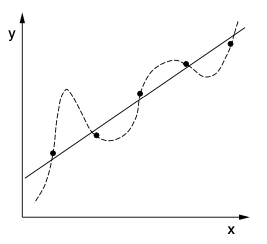
\includegraphics[width=0.5\textwidth]{Images/1.png}
    \caption{Dos posibles modelos de regresión, uno lineal y otro no, para un conjunto de datos dado.}
    \label{fig:Sobreajuste y subajuste}
\end{figure}

¿Pero qué sucede con los riesgos verdaderos \(R(f_{\text{no lineal}})\) y \(R(f_{\text{lineal}})\)? 
El problema es que no podemos calcular estos riesgos a partir de los datos de entrenamiento. 
Además, las funciones \(f_{\text{no lineal}}\) y \(f_{\text{lineal}}\) tienen comportamientos muy diferentes. 
Por ejemplo, si la línea recta \(f_{\text{lineal}}\) fuera la verdadera función subyacente, 
entonces la función discontinua \(f_{\text{no lineal}}\) tendría un riesgo verdadero elevado, 
ya que la “distancia” entre la función verdadera y la estimada es muy grande. 
Lo mismo ocurre en sentido contrario. En ambos casos, el riesgo verdadero sería mucho mayor que el riesgo empírico.


Este ejemplo resalta una decisión importante que debemos tomar: ¿preferimos ajustar los datos de entrenamiento 
con una función relativamente compleja, lo que conduce a un error de entrenamiento muy pequeño, o preferimos 
ajustarlos con una función simple a costa de un error de entrenamiento ligeramente mayor? En el ejemplo 
anterior, un físico que mida estos puntos de datos podría argumentar que no puede ser coincidencia que las mediciones 
estén casi alineadas y preferiría atribuir los residuos a errores de medición en lugar de a un modelo erróneo. Pero, 
¿es posible caracterizar en qué sentido la línea recta es más simple y por qué esto debería implicar que está, de 
alguna manera, más cerca de la verdadera dependencia subyacente? Es decir, nos interesa saber cuál es el 
aumento en el error de entrenamiento que deberíamos estar dispuestos a tolerar para ajustar un modelo más simple.

De una forma u otra, esta cuestión ha ocupado durante mucho tiempo las mentes de los investigadores que estudian 
el problema del aprendizaje. En la estadística clásica, se ha estudiado como el dilema \textit{sesgo-varianza} 
(\textit{bias-variance tradeoff}). Si ajustamos un modelo lineal para cada conjunto de datos que encontramos, 
podríamos pensar que toda dependencia funcional es lineal. Pero no sería por la naturaleza de los procesos que
generan los datos, sino un sesgo impuesto por nosotros. Por otro lado, 
si tomamos un polinomio de grado suficientemente alto para cualquier muestra, siempre podríamos ajustar 
perfectamente los datos, pero el modelo exacto que obtendríamos estaría sujeto a grandes fluctuaciones, dependiendo 
de qué tan precisas fueran nuestras mediciones en primer lugar. Esto implicaría que el modelo sufra de una gran varianza.

Una dicotomía relacionada es la existente entre el error de estimación y el error de aproximación. Si usamos una clase 
pequeña de funciones, incluso la mejor solución posible aproximará pobremente la dependencia real, mientras 
que una clase grande de funciones llevará a un error de estimación estadística alto. En la terminología del aprendizaje 
estádistico aplicado, el modelo complejo muestra \textbf{sobreajuste} (overfitting), 
mientras que el modelo lineal simple es más proclive a sufrir de \textbf{subajuste} (underfitting).

\subsection{Los dilemas sesgo-varianza y estimación-aproximación}


El ejemplo ilustrado en la Figura ~\ref{fig:Sobreajuste y subajuste}
ya señaló de manera intuitiva el problema de la complejidad del modelo: ¿cuándo un modelo es “más simple” que otro? 
¿Es bueno que un modelo sea simple? ¿Qué tan simple? 
Ya hemos mencionado anteriormente que el objetivo de la clasificación es lograr un riesgo tan bueno 
como el del clasificador de Bayes. ¿Podríamos simplemente elegir \(\mathcal{F}\) como el espacio \(\mathcal{F}_{\text{all}}\) 
de todas las funciones, definir el clasificador \(f_n := \arg\min_{f \in \mathcal{F}_{\text{all}}} \left(R_{\text{emp}}(f)\right)\), 
y obtener consistencia? Desafortunadamente, la respuesta es no. Luego veremos que, 
si optimizamos sobre clases de funciones \(\mathcal{F}\) demasiado grandes, y en particular si hacemos \(\mathcal{F}\) tan 
grande que contenga todos los clasificadores de Bayes para todas las distribuciones de probabilidad \(P\), 
esto conduce a la inconsistencia. Por lo tanto, si queremos aprender con éxito, necesitamos trabajar 
con una clase de funciones \(\mathcal{F}\) más pequeña. Para investigar las propiedades contrapuestas de la 
complejidad del modelo y la generalización, queremos introducir algunas nociones que serán útiles más adelante.

Recordemos las definiciones \(f_n\), \(f_\mathcal{F}\) y \(f_{\text{Bayes}}\) introducidas anteriormente. Hemos visto que 
la consistencia de Bayes trata sobre la convergencia del término \(R(f_n) - R(f_{\text{Bayes}})\). 
Es importante notar que podemos descomponer esta cantidad de la siguiente manera:
\[ 
\mathcal{R}(f_n) - \mathcal{R}(f_{\text{Bayes}}) = \underbrace{\mathcal{R}(f_n) - \mathcal{R}(f_\mathcal{F})}_{\text{error de generalización}} +
\underbrace{\mathcal{R}(f_\mathcal{F}) - \mathcal{R}(f_{\text{Bayes}})}_{\text{error de aproximación}} 
\]

Los dos términos en el lado derecho tienen nombres particulares: el primero se denomina 
\textbf{error de estimación} y el segundo \textbf{error de aproximación}. En la Figura 
\ref{fig:error de estimación y aproximación} 
tenemos una ilustración. El primer término aborda la 
incertidumbre introducida por el proceso de muestreo aleatorio. Dado un conjunto de datos 
finitos, necesitamos estimar la mejor función en \(\mathcal{F}\). Por supuesto, en este proceso cometeremos 
errores. Este error se denomina error de estimación. El segundo término no está influido por cantidades aleatorias.
Trata sobre el error que cometemos al buscar la mejor función en un espacio de funciones \(\mathcal{F}\) pequeño, 
en lugar de buscar la mejor función en el espacio \(F_{\text{all}}\) de todas las funciones posibles. 
La pregunta fundamental en este contexto es qué tan bien las funciones en \(\mathcal{F}\) pueden aproximar a las 
funciones en \(F_{\text{all}}\) y de allí proviene el nombre error de aproximación.

\begin{figure}[h!]
    \centering
    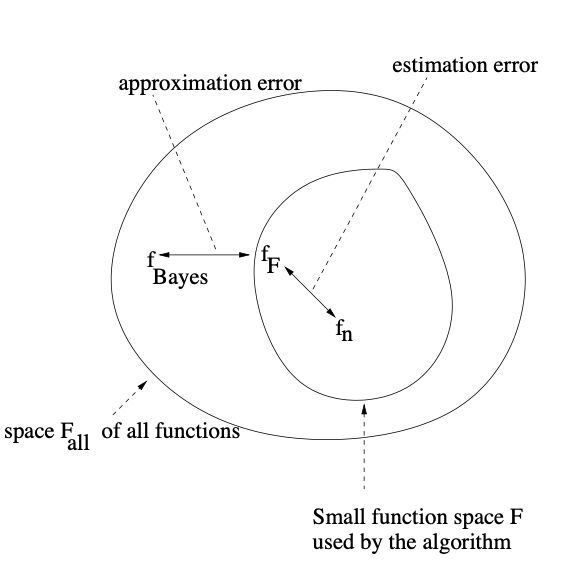
\includegraphics[width=0.5\textwidth]{Images/2.png}
    \caption{Error de estimación y de aproximación.}
    \label{fig:error de estimación y aproximación}
\end{figure}


En estadística, el error de estimación también se llama \textbf{varianza}, y el error de aproximación 
se llama \textbf{sesgo} de un estimador. Originalmente, estos términos se acuñaron para la situación 
especial de regresión con función de pérdida cuadrática, pero ahora se usan en contextos más generales, 
como el que se describe aquí. Su significado intuitivo es el mismo: el primer término mide la 
variación del riesgo de la función \(f_n\) estimada en la muestra, mientras que el segundo mide el 
sesgo introducido en el modelo al elegir una clase de funciones demasiado pequeña.

En este punto, ya podemos señalar que el espacio \(\mathcal{F}\) es el medio para equilibrar el compromiso 
entre el error de estimación y el error de aproximación. Podemos hacernos una idea gráfica viendo la Figura
. Si elegimos un espacio \(\mathcal{F}\) muy grande, el 
término de aproximación será pequeño (el clasificador de Bayes podría incluso estar contenido en 
\(\mathcal{F}\) o ser aproximado de manera cercana por algún elemento en \(\mathcal{F}\)). Sin embargo, el error de 
estimación será bastante grande en este caso: el espacio \(\mathcal{F}\) contendrá funciones complejas que 
conducirán al \textbf{sobreajuste} (overfitting). El efecto opuesto ocurrirá si la clase de funciones 
\(\mathcal{F}\) es muy pequeña.
\begin{figure}[h!]
    \centering
    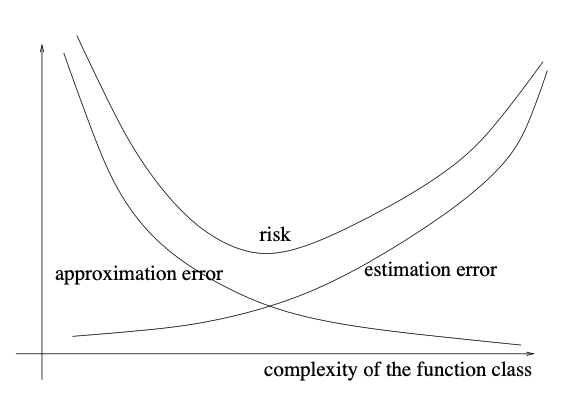
\includegraphics[width=0.5\textwidth]{Images/3.png}
    \caption{Compromiso entre error de estimación y de aproximación. Si el espacio funcional $\mathcal{F}$ que define
    el algoritmo de aprendizaje es pequeño, es decir es poco complejo, el error de estimación es bajo, pero el de aproximación
    es alto, y estamos en una situación proclive al subajuste. Si, por otro lado,  $\mathcal{F}$ es complejo, el error de estimación
    es alto y el de aproximación bajo, y tendemos al sobreajuste. El error ideal es usualmente obtenido con una complejidad moderada.}
    \label{fig:Compromiso entre error de estimación y de aproximación.}
\end{figure}

En lo que sigue, trataremos el error de estimación y el error de aproximación por separado. Veremos 
que tienen comportamientos bastante diferentes y que se necesitan métodos distintos para controlar 
cada uno.

\section{El clasificador de los $k$ vecinos más cercanos}

Hasta 1977, no se sabía si existía un clasificador universalmente consistente. 
Esta pregunta fue resuelta positivamente por Stone (1977), quien demostró, mediante una elegante prueba, 
que un clasificador particular, el denominado clasificador de los \(k\)-vecinos más cercanos 
(\textit{k-nearest neighbors classifier}, abreviado como $k$-NN), es universalmente consistente. Como el clasificador de los \(k\)-vecinos 
más cercanos es uno de los clasificadores más simples y todavía se usa ampliamente en la práctica, 
dedicaremos esta sección a ilustrar las nociones introducidas en la sección anterior, tales como 
generalización, sobreajuste, subajuste y consistencia, usando el ejemplo del clasificador \(k\)-NN.

Consideremos una muestra de puntos con etiquetas \((X_1, Y_1), \dots, (X_n, Y_n)\) que 
pertenecen a un espacio métrico. De manera general, el paradigma del aprendizaje consiste en asignar salidas 
similares a entradas similares. Es decir, creemos que los puntos que están cercanos en el espacio 
de entrada tienden a tener la misma etiqueta en el espacio de salida. Nótese que si esta afirmación 
no se cumple, el aprendizaje se vuelve muy difícil o incluso imposible. Para un aprendizaje exitoso, 
debe existir alguna forma de relacionar las etiquetas de los puntos de entrenamiento con las de los 
puntos de prueba, y esto siempre implica suposiciones previas sobre las relaciones entre los puntos 
de entrada. La relación más simple es una distancia entre puntos, pero existen otras formas de medir 
la similitud, como los \textit{kernels}, que forman la base de algunos de los algoritmos 
de aprendizaje más populares (Schölkopf y Smola, 2002).

Supongamos entonces que existe una función de distancia en el espacio de entrada, es decir, una función 
\(d : X \times X \to \mathbb{R}\), que asigna un valor de distancia \(d(X, X')\) a cada par de puntos 
de entrenamiento \(X, X'\). Dados algunos puntos de entrenamiento, ahora queremos predecir una buena 
etiqueta para un nuevo punto \(X\) que no se halla en el conjunto de entrenamiento.
 Una idea simple es buscar el punto de entrenamiento \(X_i\) 
que tenga la distancia más pequeña a \(X\) y asignar a \(X\) la etiqueta correspondiente \(Y_i\) de 
ese punto. Para definir esto de manera más formal, denotamos por \(\text{NN}(X)\) al vecino más cercano 
de \(X\) entre todos los puntos de entrenamiento, es decir:

\[
\text{NN}(X) = \arg\min \{X' \in \{X_1, \dots, X_n\} \mid d(X, X') \leq d(X, X'') \ \text{para todo} \ X'' \in \{X_1, \dots, X_n\}\}.
\]

Luego, podemos definir el clasificador \(f_n\) basado en la muestra de \(n\) puntos como:

\[
f_n(X) = Y_i \quad \text{donde} \quad X_i = \text{NN}(X).
\]

Este clasificador se denomina clasificador de un vecino más cercano (\textit{1-nearest neighbor}, 1NN). 
Podemos generalizarlo en el clasificador de los \(k\)-vecinos más cercanos (\textit{kNN}), considerando los \(k\) puntos de 
entrenamiento más cercanos, con $k>1$ en este caso, y tomando el promedio de todas sus etiquetas. 


\begin{dfn}
    Dados un espacio métrico \(X\) junto a una función de distancia \(d : X \times X \to \mathbb{R}\), 
    un conjunto de puntos de entrenamiento con sus etiquetas \((X_1, Y_1), \dots, (X_n, Y_n)\) y un entero \(k \geq 1\), 
    definimos los \textbf{\(k\)-vecinos más cercanos} de un punto \(X\) como el conjunto de los \(k\) puntos 
    de entrenamiento más cercanos a \(X\), es decir:

    \[
    \text{kNN}(X) = \{X_{i_1}, \dots, X_{i_k}\} \quad \text{donde} \quad i_1, \dots, i_k = \arg\min_{1 \leq j \leq n} d(X, X_j).
    \]
\end{dfn}

Es decir, definimos los 
\(k\)-vecinos más cercanos de \(X\), \(\text{kNN}(X)\), como el conjunto de los \(k\) puntos de 
entrenamiento más cercanos a \(X\). Luego, el clasificador \(k\)-NN se define como:

\begin{dfn}
    Con las mismas condiciones de la definición anterior,
    definimos el \textbf{clasificador de los \(k\)-vecinos más cercanos} como la función \(f_n : X \to Y\) 
    que asigna a un punto \(X\) la etiqueta que resulta de una votación mayoritaria entre las etiquetas 
    de los puntos de entrenamiento en la vecindad de \(k\)-vecinos más cercanos de \(X\):


    \[
f_n(X) = 
\begin{cases} 
+1 & \text{si } \sum_{X_i \in \text{kNN}(X)} Y_i > 0, \\ 
-1 & \text{en otro caso}.
\end{cases}
\]
\end{dfn}


Es decir, decidimos la etiqueta de \(X\) mediante una votación mayoritaria entre las etiquetas de los 
puntos de entrenamiento en la vecindad de \(k\)-vecinos más cercanos de \(X\). Para evitar empates, 
generalmente se elige \(k\) como un número impar.


\begin{thm}
    El clasificador de un vecino más cercano (1NN) no es Bayes-consistente.
\end{thm}

\begin{proof}

Consideremos 
el intervalo real \(X = [0, 1]\) y la distribución de probabilidad \(P([0, 1])\),  que asigna etiquetas 
de manera uniforme a todos los puntos \(X \in [0, 1]\) con ruido, de modo que 
\(P(Y = 1 \mid X = x) = 0.9\) para todo \(x \in X\). Es decir, la etiqueta correcta (la que 
asigna el clasificador de Bayes) es \(+1\) para todos los puntos \(x \in X\). Ya hemos mencionado 
este ejemplo cuando introdujimos el clasificador de Bayes. En este caso, el clasificador de Bayes 
es simplemente la función que devuelve \(1\) para todos los puntos en \(X\), y su riesgo Bayesiano 
con respecto a la pérdida 0-1 será

\[
\begin{aligned}
    \mathcal{R}(f_{\text{Bayes}}) & = E(\ell(X,Y,f_{\text{Bayes}}(X))) \\
    & = E(1\cdot P(f_{\text{Bayes}}(X)\neq Y) + 0 \cdot P(f_{\text{Bayes}}(X) = Y))\\
    & = E(P(f_{\text{Bayes}}(X)\neq Y))\\
    & = \int_{0}^{1} P(Y = 1 \mid X = x) \cdot \mathbb{I}_{\{f_{\text{Bayes}}(x) \neq 1\}} \, dx \\
    & \qquad \qquad + \int_{0}^{1} P(Y=0 \mid X=x) \cdot \mathbb{I}_{\{f_{\text{Bayes}}(x) = 1\}} \\
    & = \int_{0}^{1} (0.9 \cdot 0 + 0.1 \cdot 1) \, dx = 0.1.
\end{aligned}
\]

Ahora investiguemos el comportamiento del clasificador 1NN 
en este caso. Al tomar puntos de entrenamiento \((X_i, Y_i)_{i=1,\dots,n}\) de acuerdo con la 
distribución subyacente, estos estarán aproximadamente uniformemente distribuidos en el intervalo 
\([0, 1]\). En promedio, cada décimo punto tendrá una etiqueta de entrenamiento \(Y = -1\), y todos 
los demás tendrán etiqueta \(Y = +1\). Si ahora consideramos el comportamiento del clasificador \(f_n\), 
podemos escribir la probabilidad de que el clasificador 1NN cometa un error al etiqueta un punto como:

\[
\begin{aligned}
P(Y \neq f_n(X)) & = P(Y = 1 \mid f_n(X) = 0) + P(Y = 0 \mid f_n(X) = 1) \\
                 & = 0.1 \cdot 0.9 + 0.9 \cdot 0.1 \\
                 & = 2 \cdot 0.1 \cdot 0.9 = 0.18.
\end{aligned}
\]

Podemos ver que el riesgo \(R(f_n)\) del clasificador \(f_n\) es también $0,18$,
independientemente del tamaño de la muestra $n$. En efecto:

\[
\begin{aligned}
    \mathcal{R}(f_n) & = E(\ell(X,Y,f_n(X))) \\
    & = \int_{0}^{1} 1\cdot P(Y \neq f_n(X=x)) + 0 \cdot P(Y = f_n(X=x)) \, dx \\
    & = \int_{0}^{1} P(Y \neq f_n(X=x)) \, dx \\
    & = \int_{0}^{1} 0.18 \, dx = 0.18.
\end{aligned}
\]

Por otro lado el riesgo Bayesiano es $0.1$. Por lo tanto, el clasificador $1$NN no es consistente, ya que 
\(R(f_n) \not\to R(f_{\text{Bayes}})\).
\end{proof}

Consideremos por un momento el clasificador de los 100 vecinos 
más cercanos, $100$NN. En este caso, el clasificador cometería muchos menos errores que su primo de un vecino: 
es muy poco probable tener una vecindad de 100 puntos donde la mayoría de los votos sean \(Y = -1\). 
Así, el clasificador de 100 vecinos más cercanos, aunque sigue sin ser consistente, comete un error 
menor que el clasificador 1NN.

El truco para lograr consistencia está relacionado con esta observación. Esencialmente, se debe permitir 
que el tamaño \(k\) de la vecindad bajo consideración crezca con el tamaño de la muestra \(n\). Formalmente, 
se puede demostrar el siguiente teorema:


\begin{thm}[Stone, 1977]
Sea \(f_n\) el clasificador de los \(k\)-vecinos más cercanos construido 
a partir de una muestra de \(n\) puntos. Si \(n \to \infty\) y \(k \to \infty\) de modo que \(k/n \to 0\), 
entonces \(R(f_n) \to R(f_{\text{Bayes}})\) para todas las distribuciones de probabilidad \(P\). 
Es decir, la regla de clasificación \(k\)-NN es universalmente consistente con Bayes.
\end{thm}

Este teorema esencialmente nos dice que si elegimos el parámetro de vecindad \(k\) de forma que crezca 
lentamente con \(n\), por ejemplo \(k \approx \log(n)\), entonces la regla de clasificación \(k\)-NN es 
universalmente Bayes-consistente.

En las secciones anteriores mencionamos que la clase de funciones \(\mathcal{F}\) de la cual se elige el clasificador 
es un componente importante para la teoría del aprendizaje estadístico. En el caso del clasificador \(k\)-NN, 
esto no es tan obvio como lo será para los clasificadores que estudiaremos en secciones posteriores. 
Intuitivamente, se puede decir que, para un parámetro fijo \(k\), la clase de funciones \(\mathcal{F}_k\) es un espacio 
de funciones constantes por partes. Cuanto mayor sea \(k\), más grandes serán las vecindades de los \(k\)-vecinos 
y, por lo tanto, mayores serán los segmentos donde las funciones deben ser constantes. Esto significa que, 
para valores muy grandes de \(k\), la clase de funciones \(\mathcal{F}_k\) es relativamente pequeña (las funciones no 
pueden oscilar mucho). En el caso extremo de \(k = n\), la vecindad de los \(k\)-vecinos simplemente incluye 
todos los puntos de entrenamiento, por lo que el clasificador \(k\)-NN no puede cambiar su signo en absoluto; 
debe ser constante en todo el espacio de entrada \(X\). En este caso, la clase de funciones \(\mathcal{F}_k\) contiene solo 
dos elementos: la función que es constantemente \(+1\) y la función que es constantemente \(-1\).

Por otro lado, si \(k\) es pequeño, entonces \(\mathcal{F}_k\) se vuelve bastante grande (las funciones pueden cambiar sus 
etiquetas con mucha frecuencia y de manera abrupta). En los términos explicados en las secciones anteriores, 
podemos decir que si elegimos \(k\) demasiado pequeño, entonces la clase de funciones sobreajusta; 
por ejemplo, esto ocurre en el caso extremo del clasificador 1NN. Por el contrario, si \(k\) es demasiado grande, 
la clase de funciones subajusta, ya que simplemente no contiene funciones capaces de modelar los 
datos de entrenamiento.

En esta sección, solo hemos tocado los aspectos básicos del clasificador \(k\)-NN y no hemos desarrollado 
técnicas de prueba. Para un tratamiento más detallado de los aspectos teóricos de los clasificadores \(k\)-NN, 
recomendamos la monografía de Devroye et al. (1996).


\bigbreak
\pagebreak
\section{Bibliografía}

[1] \textit{Statistical Learning Theory: Models, Concepts and Results} - von Luxburg, Schölkopf (2008)

[2] \textit{The Nature of Statistical Learning Theory, second edition} - Vladimir Vapnik (2000)





\end{document}